\section{Load-Transient Response}
\label{sec:res-transient}

Load-removal tests examined secondary-bus charging by residual resonant
energy. The four captures below show switching and output-voltage response
around disconnection.

\begin{figure}[htbp]
\centering
\begin{subfigure}[t]{0.48\textwidth}
\centering
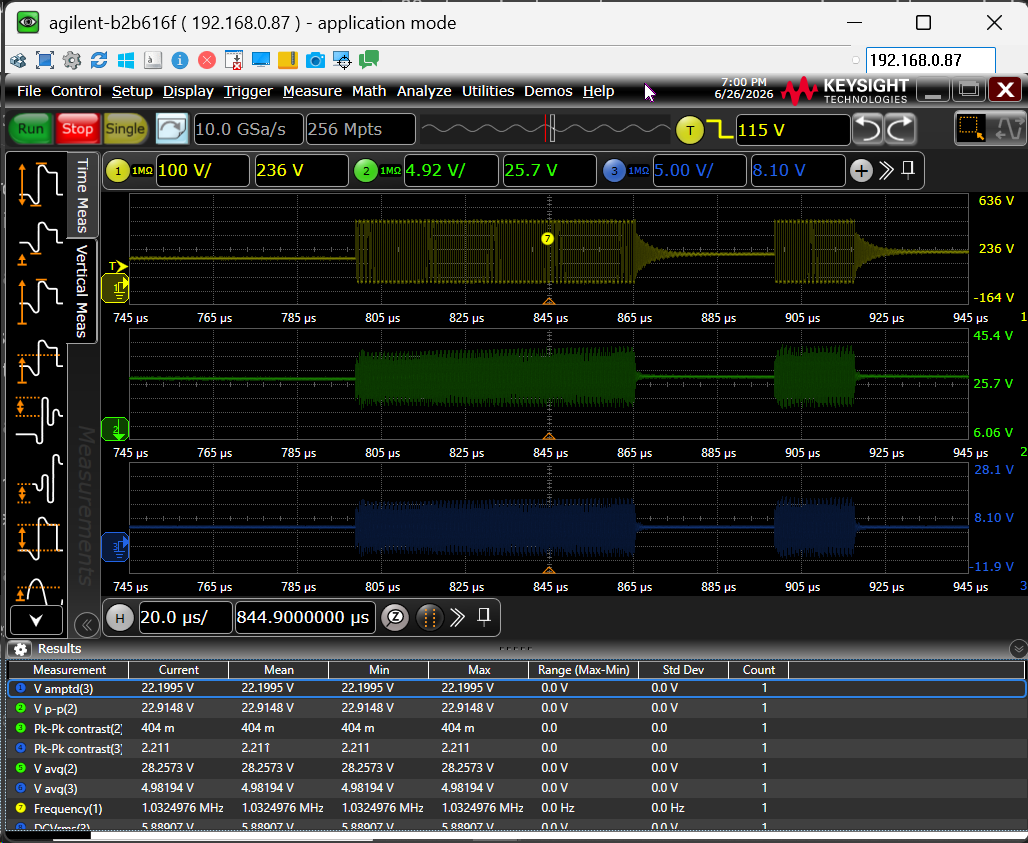
\includegraphics[width=\linewidth]{Data/measurements/evidence/PDO5_3A_to_NoLoad/keysight_5v_3a_to_no_load_sw_secondary_vbus.png}
\caption{\SI{5}{\volt}: \SI{3}{\ampere} to no load.}
\end{subfigure}\hfill
\begin{subfigure}[t]{0.48\textwidth}
\centering
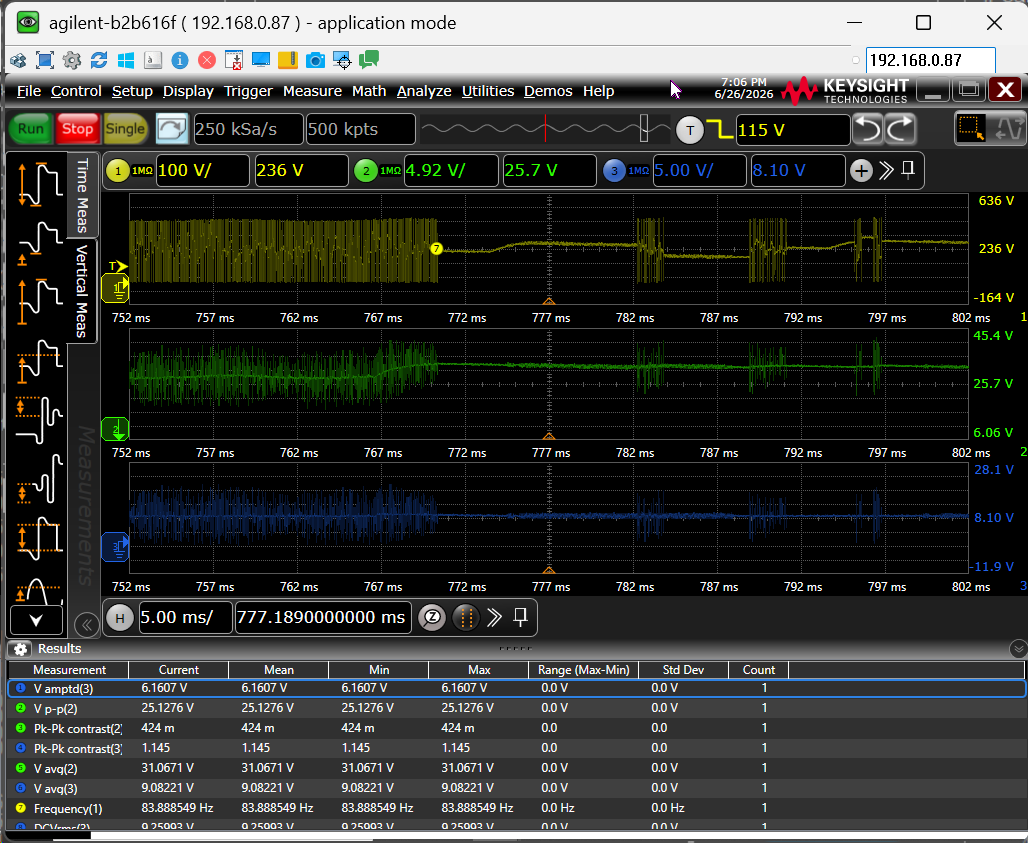
\includegraphics[width=\linewidth]{Data/measurements/evidence/PDO9_3A_to_NoLoad/keysight_9v_3a_to_0a_transient.png}
\caption{\SI{9}{\volt}: \SI{3}{\ampere} to no load.}
\end{subfigure}
\par\medskip
\begin{subfigure}[t]{0.48\textwidth}
\centering
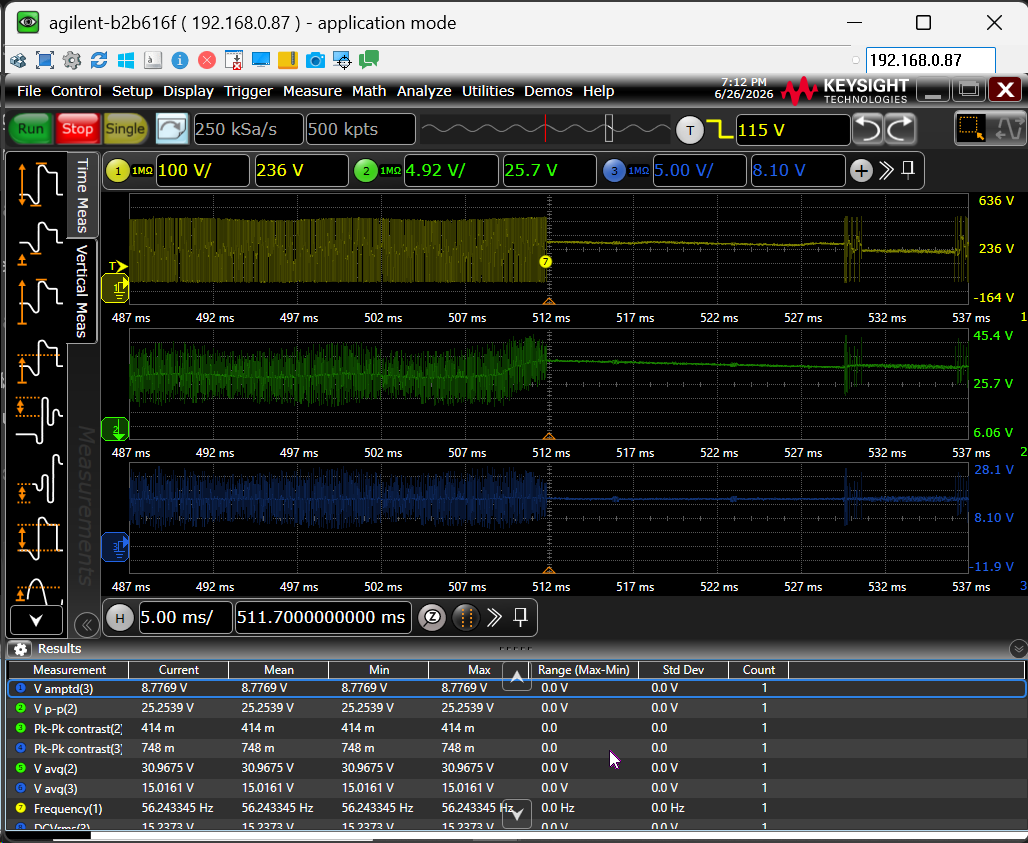
\includegraphics[width=\linewidth]{Data/measurements/evidence/PDO15_3A_TO_NL/keysight_15v_3a_to_0a_transient_sw_secondary_vbus.png}
\caption{\SI{15}{\volt}: \SI{3}{\ampere} to no load.}
\end{subfigure}\hfill
\begin{subfigure}[t]{0.48\textwidth}
\centering
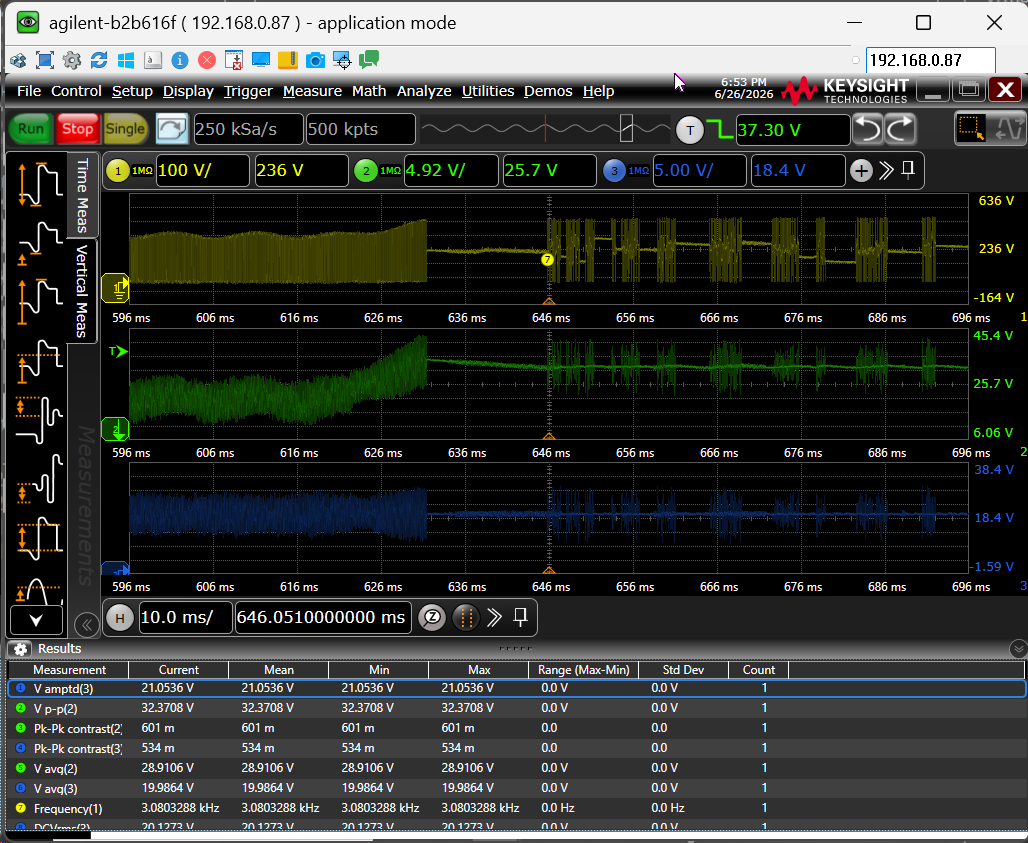
\includegraphics[width=\linewidth]{Data/measurements/evidence/PDO20_80W_to_NoLoad/keysight_80w_to_no_load_secondary_vbus.png}
\caption{\SI{20}{\volt}: nominal \SI{80}{\watt} load removal.}
\end{subfigure}
\caption{Voltage response during load removal. Yellow: half-bridge switch-node voltage. Green: secondary output voltage. Blue: USB-C VBUS output voltage.}
\label{fig:load-transient-scope-evidence}
\label{fig:load-removal-scope-evidence}
\end{figure}

\begin{table}[htbp]
\centering
\caption{Load-removal voltage readings. Average and peak-to-peak values cover the full acquisition and do not give the overshoot from the pre-step voltage.}
\label{tab:load-transient-results}
\small
\begin{tabularx}{\textwidth}{@{}L{0.26\textwidth}L{0.19\textwidth}L{0.16\textwidth}X@{}}
\toprule
Record & Transition & VBUS avg (V) & Logged VBUS pp (V)\\
\midrule
\sourcefile{PDO9-3A-TO-NL-001}, row 31 & \SI{3}{\ampere} to \SI{0}{\ampere} & 9.08221 & 1.145\\
\sourcefile{PDO15-3A-TO-NL-001}, row 35 & \SI{3}{\ampere} to \SI{0}{\ampere} & 15.0161 & 0.414\\
\bottomrule
\end{tabularx}
\end{table}

A numerical overshoot measurement would use
\begin{equation}
\Delta V_\mathrm{over}=V_\mathrm{max}-V_\mathrm{pre},
\end{equation}
using the pre-step mean and a synchronized event marker. Recovery requires
a specified regulation band. Neither result can be calculated from the
acquisition-wide pp readings. Burst-enable PA10 and UART state were not
recorded at the same time, so the response cannot be assigned to
\texttt{LBOOST}, the voltage window, or no-load guarding. Repeated steps
with event markers are needed to measure each response.
